  \subsection{Hard Ant}
    \subsubsection{Definición}
      \paragraph{Hard Ant es uno de los bloques funcionales base de Ambienta2MX, su función principal es la de enrutar las peticiones a las bases de tipo MX además de brindar la solución cartográfica (a nivel ubicación) interactuando con Fast Eagle.}
      \paragraph{Como complemento a la arquitectura, también contará con el proceso del registro masivo de información, exponiendo servicios que el módulo Smart Owl usará de forma constante para persistir la información estandarizada de diversas fuentes de información.}
      \paragraph{Hard Ant brindará los canales de acceso a las bases MX definidas en el diagrama general mediante servicios HTTP, estos servicios brindarán información para el proceso de inserción y extracción de la información. }
      \paragraph{Este módulo es lo que sería considerado la capa del modelo de datos en un patrón MVC, ya que es la que tiene contacto de forma directa con los datos almacenados en las bases de datos orientadas a documentos gestionadas por Mongo.}
      \paragraph{Se utilizará un pool de conexiones a la base para garantizar el acceso o escritura a los datos además de brindar la posibilidad de respuestas asincronas y no bloqueantes entre las consultas realizadas.}
      \paragraph{Considerando trabajos más pesados (Obtención de datos climáticos considerando un radio, cadena de búsqueda o bien información de un punto definido) se utilizarán procesos en segundo plano, esto es posible gracias a la implementación de ``Verticles'' nativas de Vert.x, tecnología que será usada para el desarrollo y despliegue final de éste módulo.}
      \paragraph{Actualmente se propone el despliegue de varias ``Verticles'', además de las que el mismo framework despliega para el consumo de las bases de datos \cite{33}.Quedando en ocho, cuatro encargadas de la comunicación y distribución de la información y las cuatro restantes para atender peticiones.} 
      \paragraph{De forma específica, también se hará uso de los canales implementados por Vert.x para generar una comunicación con las bases de datos con la finalidad de poder generar la distribución de estas. Los canales podrían ser accedidos siempre y cuando se pertenezca a la misma red o bien al cluster de Vert.x, esta modalidad no ha sido habilitada por cuestiones de seguridad.}
      \paragraph{Hablando más a detalle, Hard Ant, puede ser desplegado utilizando la línea de comandos gracias a las funciones que nos provee Gradle, framework utilizado para el maquetado, resolución de dependencias y gestión de tareas del proyecto. \cite{34}}
      \newpage
        \begin{landscape}
          \subsubsection{Diagrama de Clases}
          \paragraph{A continuación se mostrará el de clases que define la estructura de Hard Ant.}
          \begin{figure}[b!]
          \centering
          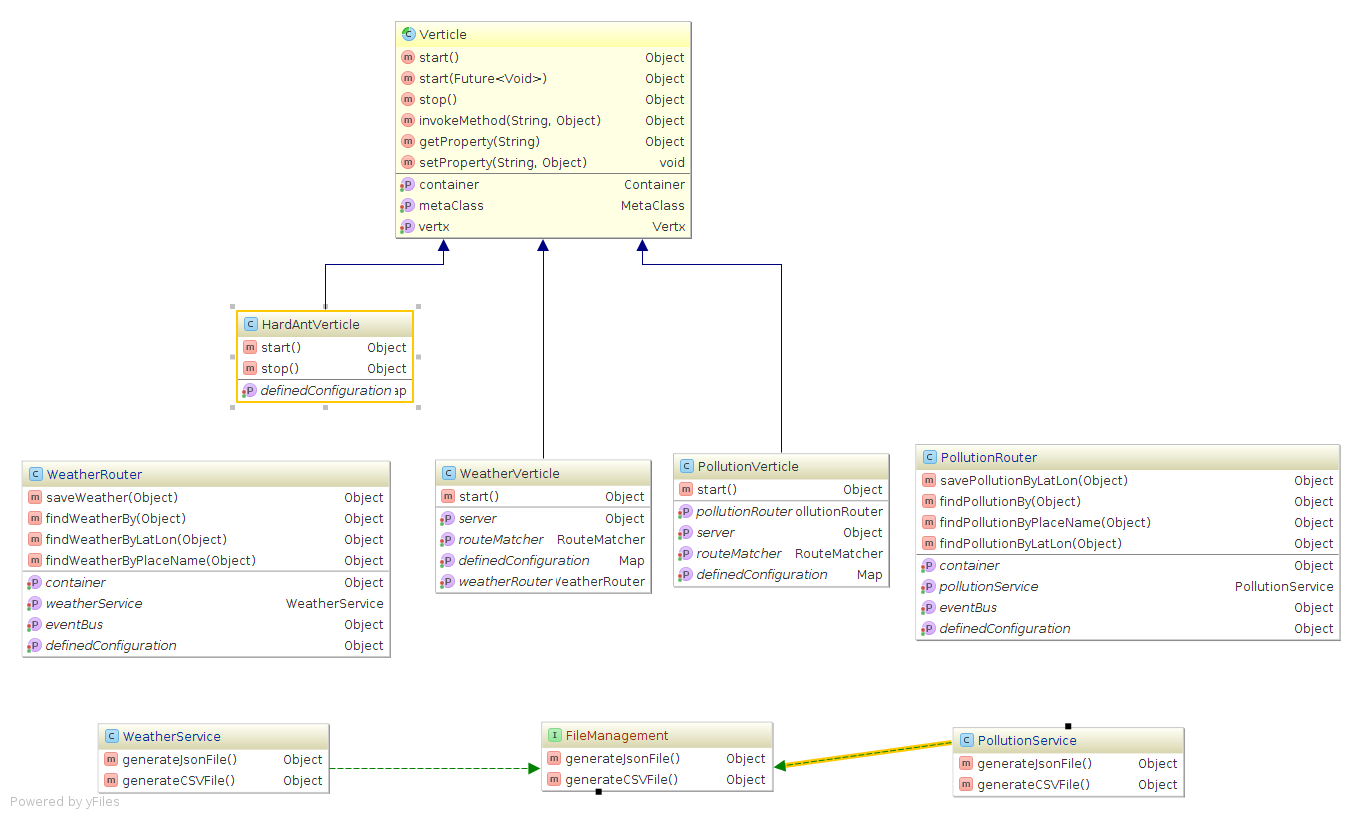
\includegraphics[width=17.5cm,height=12cm]{./images/HardAntClassDiagram.png}
          \caption{Diagrama de clases de Hard Ant}
        \end{figure}
        \end{landscape}
      \newpage
      \newpage
        \begin{landscape}
          \subsubsection{Diagrama por bloques}
          \paragraph{A continuación se muestra el diagrama a bloques que define la funcionalidad de Hard Ant.}
          \begin{figure}[b!]
          \centering
          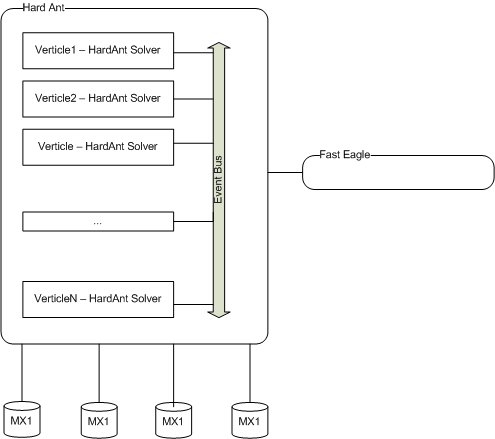
\includegraphics[width=17.5cm,height=12cm]{./images/DiagramaHardAnt.png}
          \caption{Diagrama a bloques de Hard Ant}
        \end{figure}
        \end{landscape}
      \newpage
    \paragraph{En el diagrama se puede apreciar la replicación de ``Verticles'' que interactuan a través del mismo canal de información, esto brinda disponibilidad del servicio ya que las peticiones son atendidas y procesadas no sólo por un elemento existente si no varios. La interacción con este servicio se realizará utilizando servicios REST, utilizando el módulo de Cute Bunny como medio de comunicación con la vista que tendrá el usuario final.}
    \paragraph{Este módulo se puede encontrar en cualquier otra máquina, debido al método de comunicación utilizado entre los módulos, sólo basta con realizar la configuración de las direcciones o dominios donde se encuentra alojado para qué este puede pueda ser accedido.}